
\subsection{Spark use-case}

\begin{itemize}
\item description of the use-case and its Madeus commissioning
\item experimental setup
\item results and comparison to theoretical perf
\end{itemize}

\subsection{OpenStack use-case}
\label{subsec:openstack}

\subsubsection{Presentation}

OpenStack~\cite{os:7923796} is the de-facto open-source solution to address the
IaaS level of the Cloud paradigm. Since $2010$, its community has gathered
nearly $700$ organizations (such as Google, IBM or Intel) and has produced more
than $20$ million lines of code. Its adoption is still growing in various
domains such as public administrations, e-commerce and science\footnote{See
\url{http://superuser.openstack.org/} for further information.}.

OpenStack is a large distributed software that brings together almost $100$
software projects. Each project is in charge of a specific aspect of the
infrastructure management (e.g. managing virtual machines, providing them with
storage, connecting them through networks) whose cooperation is the key to
provide the features required for Cloud management. Furthermore, those projects
are themselves composed of several modules that are responsible for very
specific tasks. While they are not all mandatory to deploy an operable IaaS,
$250$ modules are contained in those projects. An OpenStack instance is a
selection of those modules that cooperate to respond to the operator's
requirements. The deployment of an OpenStack instance implies thus many tasks
and interplays that are complex to understand. As a consequence, the deployment
of OpenStack is a tedious challenge to handle manually on large-scale
infrastructures.%~\cite{bell2015jop}.

\begin{table*}
  \begin{center}
    
\begin{tabular}{|c|c|c|c|c|}
   \hline
   & Roles & Places & Transitions & Ports \\
   \hline
   Nova & Manages compute instances (\eg Virtual machines) & 5 & 8 & 8\\
   Glance & Compute image store & 3 & 4 & 7\\
   Neutron & In charge of network resources & 3 & 4 & 7\\
   MariaDB & An SQL server used by most projects to store persistent
    information & 4 & 5 & 4\\
   Keystone & Manage user authentication, authorization and service
    discovery & 3 & 2 & 4\\
   RabbitMQ & The message bus for inter-service communication & 2 & 1 & 3\\
   HAProxy & Load-balances the requests to OpenStack controllers & 2 & 1 & 7\\
   OpenVSwitch & Virtualizes network functions & 3 & 1 & 2\\
   MemCached & Caches ephemeral data for most OpenStack projects & 2 & 1 & 2\\
   Facts & Collects informations about every nodes & 2 & 1 & 1\\
   Common & Common utilities (\eg cron, fluentd: a metric collector for logging)
    & 3 & 2 & 2\\
%   \hline
%   Total & 32 & 30 & 47 & \\
%   \hline
%   & Places & Transitions & Ports & Roles\\
%   \hline
%   Nova & 5 & 8 & 8 & Manage compute instances (\eg Virtual machines)\\
%   Glance & 3 & 4 & 7 & Compute image store\\
%   Neutron & 3 & 4 & 7 & In charge of network resources\\
%   Keystone & 3 & 2 & 4 & Manage user authentication, authorization and service
%    discovery\\
%   MariaDB & 4 & 5 & 4 & An SQL server used by most projects to store persistant
%    information\\
%   RabbitMQ & 2 & 1 & 3 & The message bus for inter-service communication\\
%   HAProxy & 2 & 1 & 7 & Load-balances the requests to OpenStack API services\\
%   OpenVSwitch & 3 & 1 & 2 & Virtualizes network functions\\
%   MemCached & 2 & 1 & 2 & Caches ephemeral data for most OpenStack projects\\
%   Facts & 2 & 1 & 1 & Collects inforamtions about every nodes\\
%   Common & 3 & 2 & 2 & Common utilities (\eg cron, fluentd: a
%   metric collector for logging) \\
   \hline
   Total & & 32 & 30 & 47\\
   \hline
\end{tabular}


    \caption{Number of places, transitions, ports and roles for each \mad component
        of the OpenStack assembly of Figure~\ref{fig:full}.} \label{tab:os}
  \end{center}
\end{table*}

In the rest of this section, \kolla will be our reference. \kolla is one of the
most popular project for deploying OpenStack in production. It relies on Ansible to
deploy OpenStack's modules as Docker containers. It is highly opinionated out of
the box, allowing operators to quickly deploy a basic OpenStack instance, but
makes complete customization possible for advanced operators. As a consequence,
the use case described in this section corresponds to the basic \kolla
deployment, which provides the essential mechanisms to operate an infrastructure
with OpenStack. Based on the roles defined in \kolla's playbooks, we have
defined $11$ \mad components whose names are for most of them, based on the
OpenStack project they deploy. \Cref{tab:os} lists these components and
indicates which aspect of the Cloud management they are in charge of, as well as
some \mad metrics: the number of places, transitions and ports. When the number
of transitions is greater or equal to the number of places, it means we were
able to leverage \mad to express parallel transitions. Also, the more ports, the
more \mad is able to coordinate interplays during the deployment. As depicted in
\cref{tab:os}, Nova, Glance, Neutron and MariaDB are of particular interests
since they contain more places, transitions and ports than the others.

\begin{figure}
  \begin{center}
    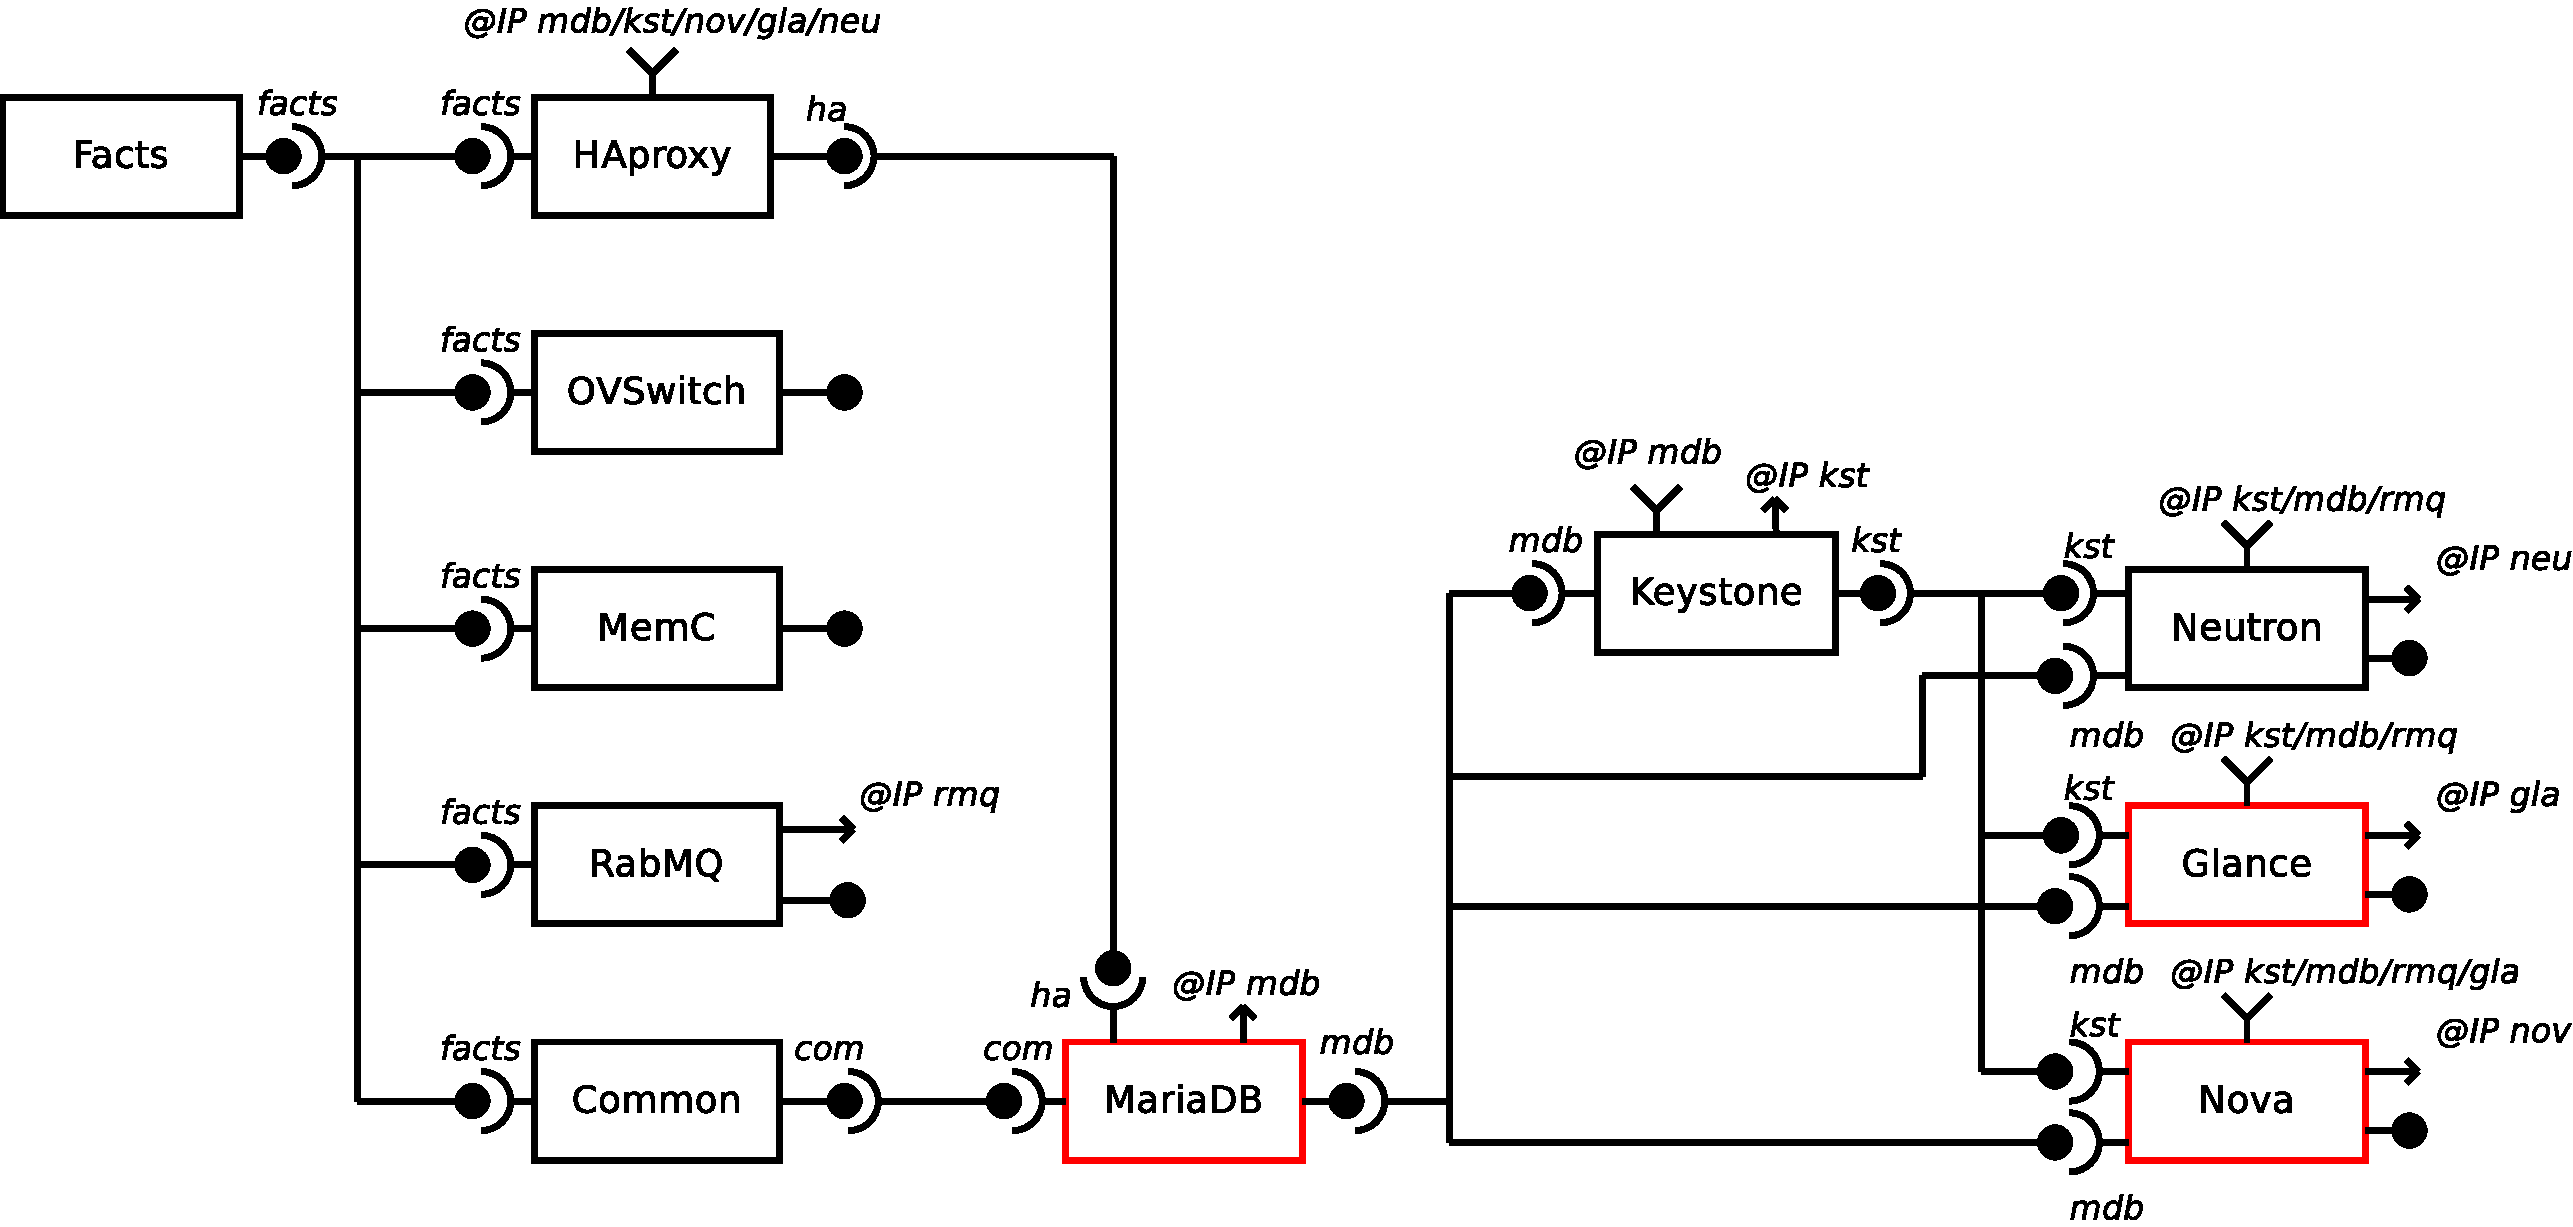
\includegraphics[width=0.5\textwidth]{./images/full.pdf}
    \caption{Simplified \mad assembly of the \kolla-based OpenStack
    deployment containing $11$ components. Red components are detailed
    in Figure~\ref{fig:sub}.}
    \label{fig:full}
  \end{center}
\end{figure}

\Cref{fig:full} depicts the use-case from the operator viewpoint, at the level
of the \mad assembly. For the sake of simplicity and readability, some
connections are not represented in this figure. This figure helps to understand
the interplays between components. For instance, Neutron, Glance and
Nova require the service catalog Keystone to be available in order to register
themselves inside the catalog. Keystone requires itself a database (\ie
MariaDB) during its deployment.
%MariaDB relies itself on HAProxy for being reachable through a virtual IP address.
However, regarding the separation of concerns, the operator does not need to
understand the internals of these components. She just needs to instantiate
them, and creates the appropriate connexions. Also, she could decide to replace
MariaDB with MySQL: another component offering a database, with the same
interfaces as MariaDB.

\begin{figure*}[t]
  \begin{center}
    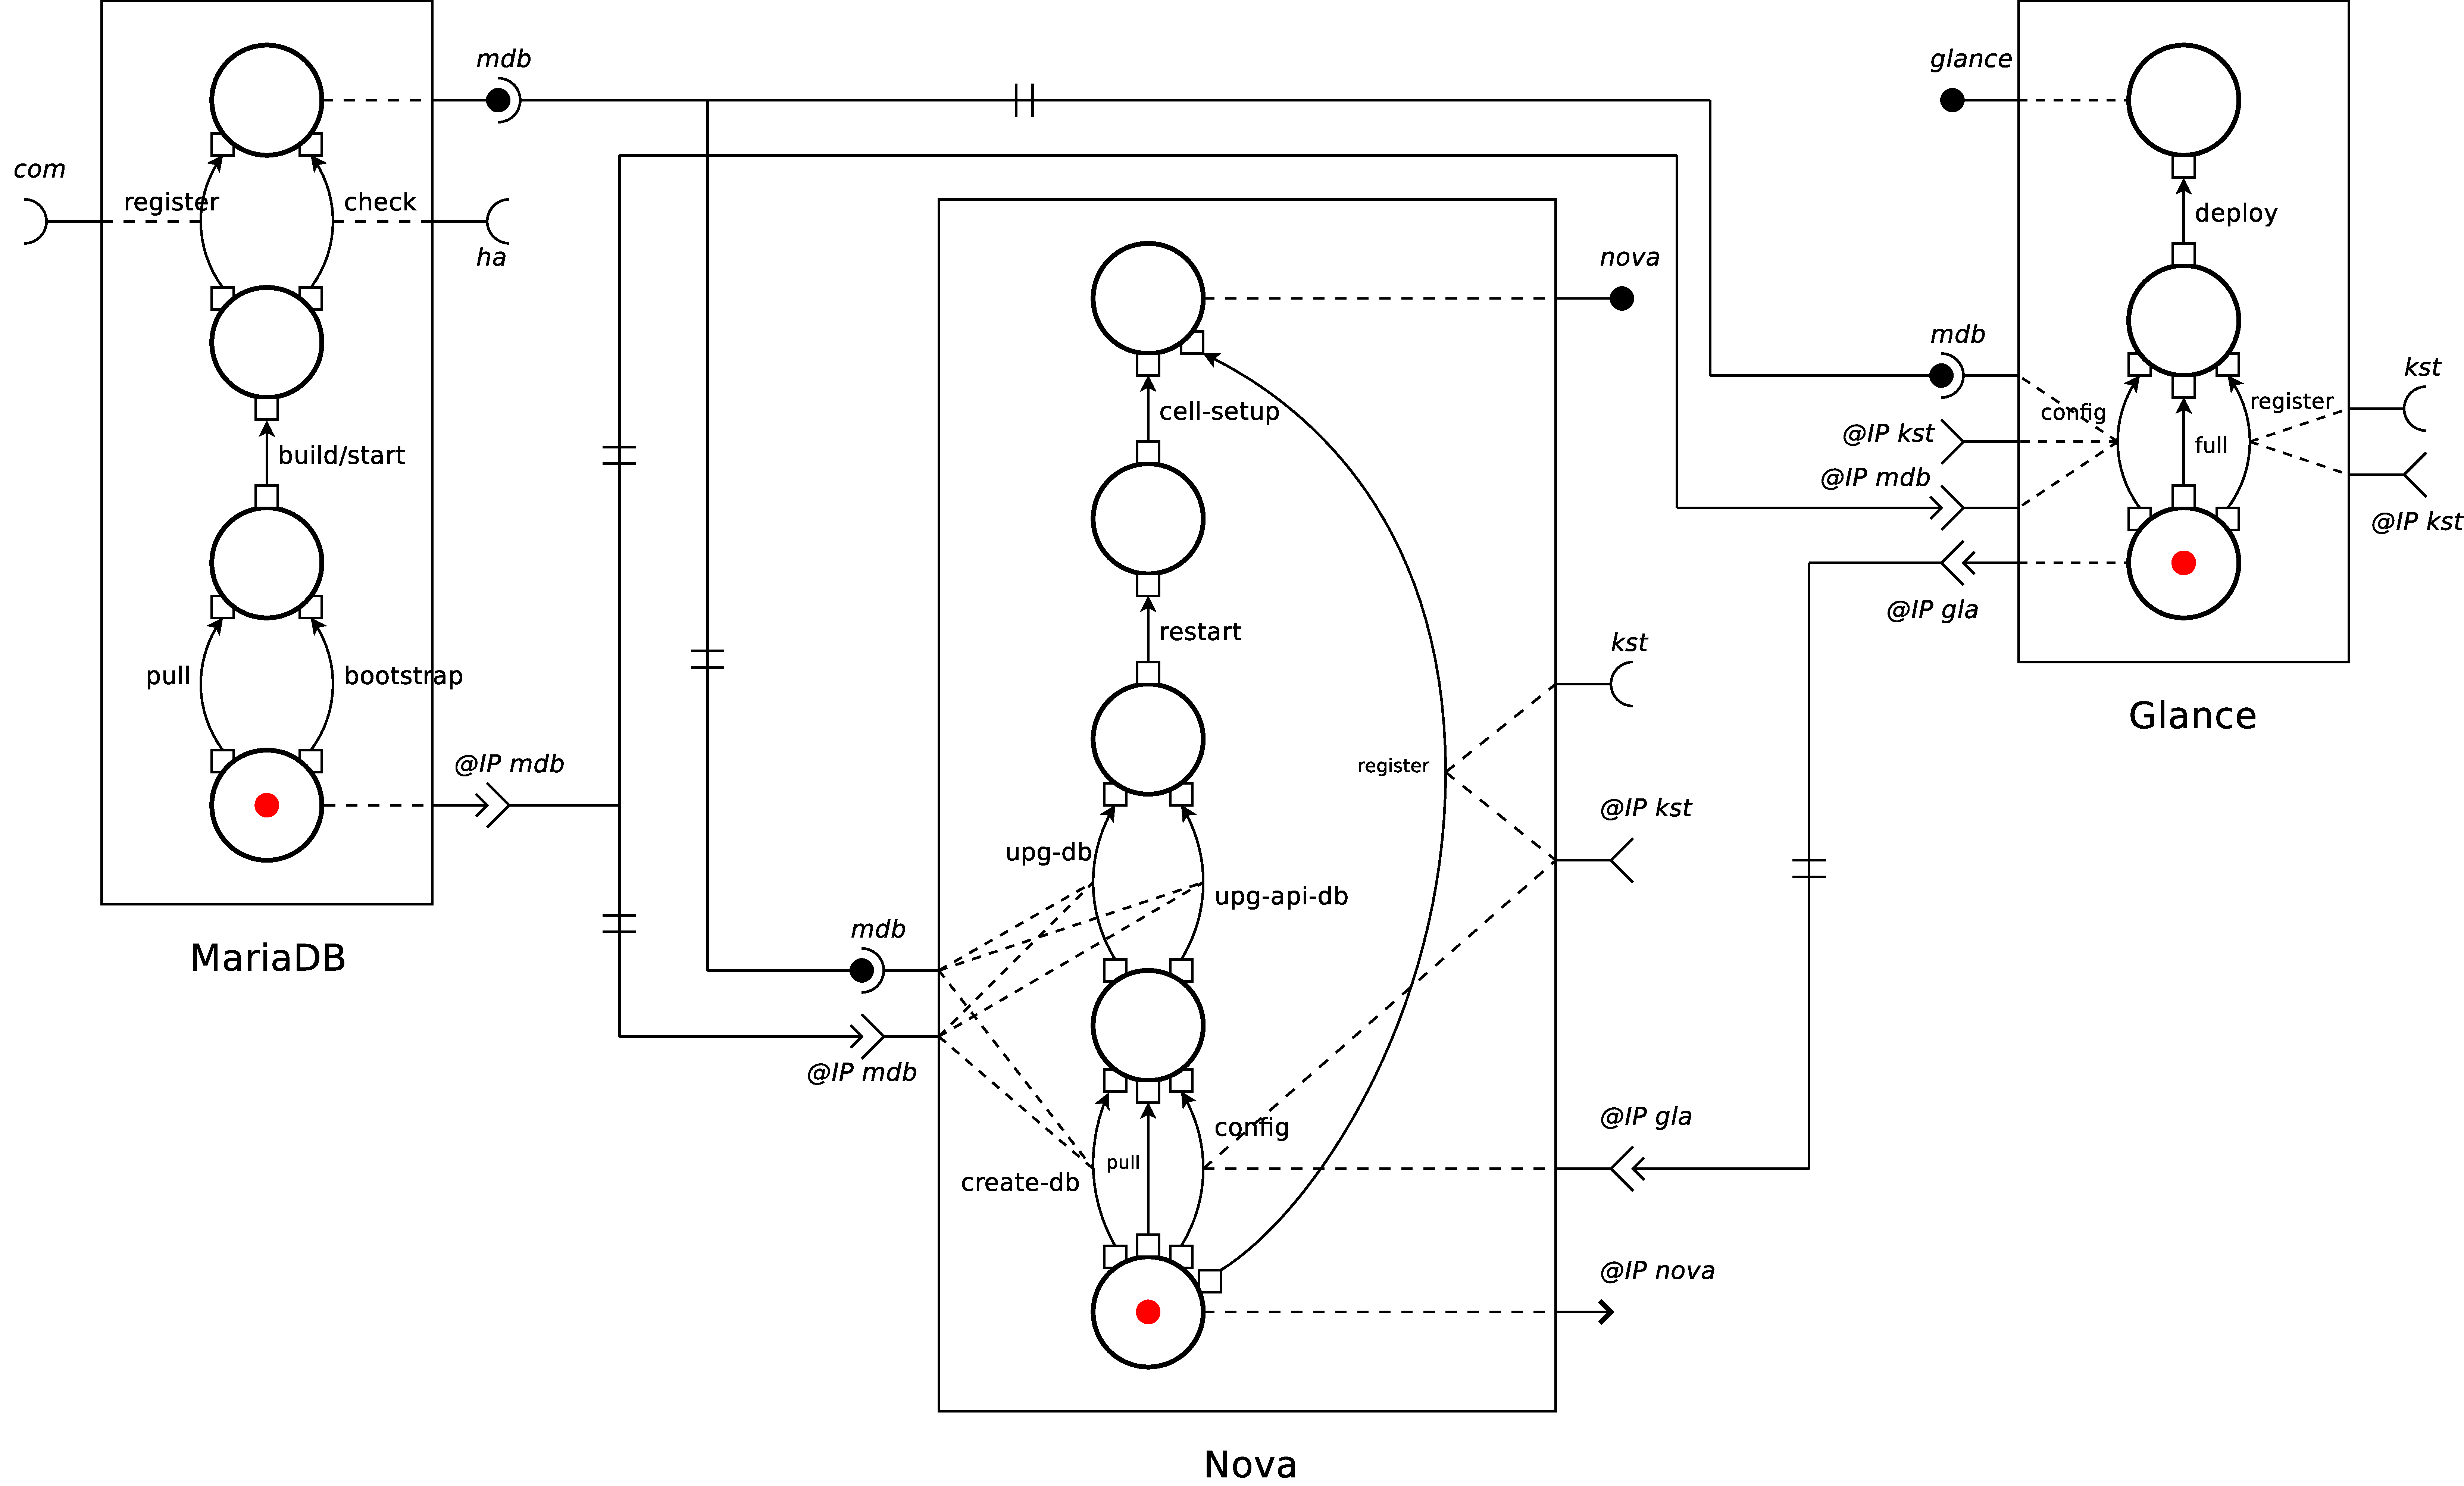
\includegraphics[width=0.8\textwidth]{./images/sub.pdf}
    \caption{A detailed sub-part of the full component assembly to deploy
    OpenStack. The three colored components of \cref{fig:full} are
    detailed by using \mad. Black, green, blue and red tokens represent
    different scenarios during the deployment process.}
    \label{fig:sub}
  \end{center}
\end{figure*}

In the following, we study our use-case from the developer viewpoint, using the
three colored components from \cref{fig:full}: MariaDB, Nova and Glance. 
\Cref{fig:sub} depicts the internals of these components and how they are
connected.
%
First, one can note from this figure that the MariaDB component is different
from the one depicted in \cref{fig:run0}. The component here difference has
additional content: (i) the transition \emph{register} that relies on the Common
component; (ii) the transition \emph{check} that relies on the HAProxy (in our
use-case, MariaDB is reachable from HAProxy's virtual IP address).  This
illustrates that according to the type of deployment the developer or the
operator aims at performing, the internal life cycle of a component may need to
be modified. Thus, it shows that being able to customize a component life cycle
may be needed to improve both the expressiveness and efficiency of a deployment.

Second, the dependencies previously observed at the assembly level are relaxed
and more detailed at the internal level. If we isolate Nova and Glance for
instance, while we could believe in \cref{fig:full} that Glance must be deployed
before Nova, it is clear here that once Nova obtains Glance's IP address
(provided by the first place in Glance), both components can be deployed in
parallel.

Third, this example shows how \mad can be leveraged to express both inter and
intra-component parallelism. Nova defines four parallel branches after its first
place that are merged at two distinct places. Three of them are merged at the
next place, while one of them is joined much later after the transition
\emph{cell-setup}. Hence, \mad is more expressive than a fork-join model.

%Moreover, one can note in this example that provide ports (data) can be
%connected to multiple use ports (data), and that use ports (data) can
%be bound to multiple transitions in \mad.
%
%Finally, as illustrated by both examples of Figures~\ref{fig:run}
%and~\ref{fig:sub}, \mad is able to model any kind of service,
%corroborating software \emph{Genericty} (\emph{soft-gen}
%metric). Similarly, as any set of actions can be performed within a
%transition, any kind of resource could be used with \mad (\eg bare
%metal or virtualized environments), ensuring the resource genericity
%of our solution. While this property is not new compared to existing
%solutions, it is preserved by \mad.

\subsubsection{Experimental Setup}
% Ici on décrit nos paramètres et le testbed

This section compares three different OpenStack deployments. The first one,
called \emph{spmd-1t}, corresponds to a sequential assembly of components whose
life cycles are based on a single transition (\emph{1t}). Concretely,
\emph{spmd-1t} matches the \kolla-ansible deployment process.
%The assembly is similar to the one presented in Figure\ref{fig:benchA}.

The second OpenStack deployment, called \emph{dag-2t}, describes a dependency
Directed Acyclic Graph (\emph{dag}) of components, which are thus deployed in
parallel according to their ports bound to their internal transitions. Regarding
components' internals, they are based on two sequential transitions (\emph{2t}).
This deployment assembly is equivalent to an Aeolus deployment of OpenStack,
with fine-grained parallelism at the component level, and no parallelism at the
task level.

Finally, the third OpenStack deployment, called \emph{dag-nt}, represents a
\emph{dag} assembly of components where components life cycles are customised by
$n$ transitions (\emph{nt}), in parallel when possible. In this definition, both
components and transitions are run in parallel, which corresponds to a
contribution of our \mad model.

We now study the resources and the module distribution in our setup. Since
OpenStack projects contain multiples modules, each of the $11$ components
defined previously deploys different modules ($36$ in total). A basic multi-node
\kolla deployment targets 3 nodes: the \emph{Control} node which hosts control
services, APIs and databases ($16$ services); the \emph{Network} node that hosts
network agents and HAProxy ($11$ services); and the \emph{Compute} node, in
charge of compute services, where guest VMs live ($9$ services).

Our evaluations have been conducted on the experimental platform
Grid'5000\footnote{\url{www.grid5000.fr}}, more precisely on four different
clusters of the platform detailed in \cref{tab:g5k}. To produce reproducible
experiments we also have used the Execo
framework\footnote{\url{http://execo.gforge.inria.fr/doc/latest-stable/index.html}}
combined with the KaDeploy bare metal environment of Grid'5000. Each result
corresponds to the average deployment time (in seconds) recorded from $10$
iterations.

\begin{table}
  \begin{center}
    \small
    
\begin{tabular}{|c|c|c|c|}
   \hline
   Cluster & CPU & Memory & Network\\
   \hline
   Nova & 2 x Intel Xeon E5-2620 v4 & 64GB & 10Gbps\\
   (lyon) & 8 cores/CPU &  & \\
   \hline
   Taurus & 2 x Intel Xeon E5-2630 & 32GB & 10Gbps\\
   (lyon) & 6 cores/CPU & & \\
   \hline
   Sol & 2 x AMD Opteron 2218 & 4GB & 1Gbps\\
   (sophia) & 2 cores/CPU & &\\
   \hline
\end{tabular}


    \caption{Grid'5000 cluster configurations.}
    \label{tab:g5k}
  \end{center}
\end{table}

As previously said, \kolla-ansible (\ie \emph{spmd}) is our reference in this
use-case.  To ease our work, we re-use the playbooks already provided by \kolla
by splitting them in the transitions of \mad components. Since \kolla presupposes
the resources have been provisioned before running it, we do not consider this
phase during in this use-case (even if it could be managed by \mad).
%
Also, since \kolla relies on Docker containers, fetching Docker images has a
significant impact on our results: images have to downloaded before being
decompressed. To be as neutral as possible we have conducted experiments with
three different ways for handling those images: (1) \emph{cached} in which
images are previously placed on OpenStack nodes, so that fetching Docker images
has no impact on our results; (2) \emph{local} where images are previously
downloaded on a dedicated node of the cluster from which images can be loaded (a
local Docker registry); (3) \emph{remote} in which images are available from an
Internet repository (\ie the DockerHub registry).  \Cref{tab:images} gives for
each OpenStack node (\ie Compute, Network and Control) the number of Docker
images to download and their compressed size.

\begin{table}
  \begin{center}
    
\begin{tabular}{|c|c|c|c|}
   \hline
   & Compute & Network & Control\\
   \hline
   Number of images & $9$ & $11$ & $16$\\
   \hline
   Total Size (MB) & $2767$ & $2705$ & $4916$\\
   \hline
\end{tabular}


    \caption{Number of Docker images per node and their cumulated size in MB to
      download from the registry.}
    \label{tab:images}
  \end{center}
\end{table}

\subsubsection{Results}

